\subsection{Satz von Taylor}
Wir sehen uns noch einmal die Formel aus dem Mittelwertsatz der Differentialrechnung an.
\begin{equation*}
	f(b)-f(a)=(b-a)*f'(\xi)
\end{equation*}
Wir setzen jetzt $b=x$ und $a=x_0$ und erhalten damit:
\begin{equation*}
	f(x)=f(x_0)+(x-x_0)*f'(\xi)
\end{equation*}
Um eine Approximation von $f$ in der Nähe von $x_0$ zu erhalten, ersetzen wir in der obigen Formel $\xi$ durch $x_0$. Wir erhalten dann:
\begin{equation*}
	f(x)\approx f(x_0)+(x-x_0)*f'(x_0)
\end{equation*}
Wir ersetzen also näherungsweise die Funktion $f$ durch das Lineare Polynom, dessen Graph die Tangente an den Graph von $f$ bei $x_0$ ist.

Diese Funktion $T_1(x)=f(x_0)+(x-x_0)*f'(x_0)$ wird als das \emph{Taylorpolynom} ersten Grades von $f$ bei $x_0$ bezeichnet. Die Funktion $T_1$ ist dadurch gekennzeichnet, dass ihre erste und nullte Ableitung mit der ersten und nullten Ableitung von $f$ bei $x_0$ übereinstimmen. Das heißt:
\begin{align*}
	T_1(x_0)&=f(x_0)\\
	T_1'(x_0)&=f'(x_=)
\end{align*}
Wir führen nun das $n$te Taylorpolynom ein, indem wir fordern, dass es am Punkt $x_0$ mit der Funktion $f$ in der nullten bis zur $n$ten Ableitung übereinstimmt.

Nun stellt sich die Frage nach der Güte der Approximation.

\begin{lemma}{Taylorpolynom}
	Sei $f$ $n$-mal differenzierbar im Intervall $(a,b)$ und $x_0\in(a,b)$. Dann gibt es genau ein Polynom $n$ten Grades $T_n$, so dass gilt
	\begin{equation}\label{eq:taylorpolynom}
		T_n^{(k)}(x_0)=f^{(k)}(x_0) \quad\forall k\in[0,n]\in\N
	\end{equation}
	Dieses Polynom wird Taylorpolynom $n$ten Grades von $f$ um den Entwicklungspunkt $x_0$ genannt.
	Dabei ist
	\begin{align*}
		T_n(x_0)&=\sum\limits_{j=0}^n \frac{f^{(j)}(x_0)}{j!}(x-x_0)^j\\
		&=\underbrace{f(x_0)+f'(x_0)*(x-x_0)}_{=T_1}+\ldots+\frac{f^{(k)}(x_0)}{n!}(x-x_0)^n
	\end{align*}
\end{lemma}
\beweis
Wir zeigen zunächst die Eindeutigkeit. Seien $P,Q$ Polynome, die die Eigenschaften aus \autoref{eq:taylorpolynom} besitzen.
Für die Differenz $D=P-Q$ gilt:
\begin{equation*}
	D(x)=P(x)-Q(x)=b_0+b_1*x+\ldots+b_n*x^n
\end{equation*}
Wobei $D^{(k)}(x_0)=0$ für alle $0\leq k\leq n$. Es folgt also
\begin{equation*}
	D^{(n)}(x_0)=n!*b_n=0\enspace \rightsquigarrow b_n=0
\end{equation*}
Im nächsten Schritt sehen wir
\begin{equation*}
	D^{(n-1)}(x_0)=(n-1)!*b_{n-1}=0\enspace \rightsquigarrow b_{n-1}=0
\end{equation*}
und so weiter.
Am Ende sehen wir, dass alle $b_k=0$ sind, dies zeigt die Eindeutigkeit.

Man rechnet leicht nach, dass $T_n^{(k)}(x_0)=f^{(k)}(x_0)$ gilt.\hfill$\Box$

\paragraph{Bemerkung:}
Die Potenzreihe
\begin{equation*}
	\sum\limits_{n=0}^\infty \frac{f^{(n)}(x_0)}{n!}(x-x_0)^n
\end{equation*}
für eine beliebig oft differenzierbare Funktion $f$ wird auch die Taylorreihe von $f$ um $x_0$ genannt.

\paragraph{Beispiele:}
\begin{itemize}
	\item Sei $f$ die Exponentialfunktion $f=e^x$, dann gilt $f^{(k)}(x_0)=e^x$ für alle $k$. Damit gilt für das $n$te Taylorpolynom von $e^x$ bei $x_0=0$: $f^{(k)}(0)=e^0=1$.
	\begin{equation*}
		T_n(x)=1+\frac{1}{1!}x+\frac{1}{2!}x^2+\frac{1}{3!}x^3+\ldots +\frac{1}{n!}x^n
	\end{equation*}
	Das gilt also, dass die Taylorreihe von $e^x$ bei $x_0=0$ mit der Exponentialreihe übereinstimmt.
	\item Sei $f(x)=\sin(x)$ und $x_0=0$. Es gilt:
	\begin{align*}
		f^{(0)}(0)&=\sin(0)=0 & f^{(1)}(0)&=\cos(0)=1\\
		f^{(2)}(0)&=-\sin(0)=0 & f^{(3)}(0)&=-\cos(0)=-1
	\end{align*}
	Also folgt $f^{(2k)}(0)=0$ und $f^{(2k+1)}(0)=(-1)^k$.
	Damit erhalten wir für das Taylorpolynom:
	\begin{equation*}
		T_{2n+1}=\underbrace{x-\frac{1}{3!}x^3+\frac{1}{5!}x^5-\frac{1}{7!}x^7}_{T_7(x)}\pm\ldots+\frac{1}{(2n+1)!}x^{2n+1}
	\end{equation*}
	Hieraus folgt, dass die Taylorreihe von $\sin(x)$ bei $x_0=0$ genau die Potenzreihe von $x\mapsto\sin(x)$ ist, mit der wir den Sinus definiert haben.

	Bereits das Taylorpolynom dritten Grades nähert den Sinus im Intervall $[-\pi,\pi]$ gut an:
	\begin{center}
		\begin{easyfunction}{-5}{5}{-1}{2.5}{1}
			\draw[->] (-5.2,0) -- (5.2,0) node[right] {$x$};
			\draw[->] (0,-2) -- (0,2) node[above] {$f(x)$};
			%\makegrid
			\draw (3.1415,0) node (a) [fill = white,rectangle,inner sep = 0pt,minimum size = 0pt,minimum height=4pt,draw, label={below:$\pi$}] {};
			\draw (1.5707,0) node (a) [fill = white,rectangle,inner sep = 0pt,minimum size = 0pt,minimum height=4pt,draw, label={below:$\frac\pi2$}] {};
			\draw (-3.1415,0) node (b) [fill = white,rectangle,inner sep = 0pt,minimum size = 0pt,minimum height=4pt,draw, label={below:$-\pi$}] {};
			\draw (-1.5707,0) node (a) [fill = white,rectangle,inner sep = 0pt,minimum size = 0pt,minimum height=4pt,draw, label={below:$-\frac\pi2$}] {};

			\begin{scope}
				\clip (-5,-1.5) rectangle (5,1.5);
				\draw[line width=0.5mm,scale=1,domain=-5:5,smooth,variable=\x,blue] plot ({\x},{sin(deg(\x))})
					node[above left] {$\sin(x)$};
				\draw[line width=0.3mm,scale=1,domain=-3.9:3.9,smooth,variable=\x,green] plot ({\x},{\x-1/6*\x*\x*\x+1/120*\x*\x*\x*\x*\x})
					node[below right] {$T_5(x)$};
				\draw[line width=0.3mm,scale=1,domain=-3.9:3.9,smooth,variable=\x,red] plot ({\x},{\x-1/6*\x*\x*\x+1/120*\x*\x*\x*\x*\x-1/5040*\x*\x*\x*\x*\x*\x*\x})
					node[left] {$T_7(x)$};
			\end{scope}
		\end{easyfunction}
	\end{center}
\end{itemize}

Um die Güte der Approximation durch Taylorpolynome abschätzen zu können, benutzen wir den folgenden Satz:
\begin{satz}{Satz von Taylor}
Sei $f$ eine $n+1$ mal stetig differenzierbare Funktion auf $(a,b)$ und seien $x,x_0\in(a,b)$. Dann existiert ein $\xi\in(x,x_0)$ beziehungsweise ein $\xi\in(x_0,x)$, so dass gilt:
\begin{equation*}
	f(x)=T_n(x)+\underbrace{\frac{f^{(n+1)}(\xi)}{(n+1)!}(x-x_0)^{n+1}}_{\text{LaGrange'sches Restglied}}
\end{equation*}
\end{satz}
\beweis
Wir betrachten ein festes $x$ und ein variables $t$ und sehen:
\begin{equation*}
	F(t)=f(x)-f(t)-f'(t)(x-t)-\frac{f''(t)}{2!}(x-t)^2-\ldots-\frac{f^{(n)}(t)}{n!}(x-t)^n
\end{equation*}
\begin{equation*}
	G(t)=\frac{(x-t)^{n+1}}{(n+1)!}
\end{equation*}
Es ist $F(x_0)=f(x)-T_n(x)$ und $F(x)=G(x)=0$. Weiterhin gilt:
\begin{align*}
	F'(t)&=-f'(t)-f''(t)(x-t)-\frac{f'''(t)}{2!}(x-t)^2-\ldots-\frac{f^{(n+1)}(t)}{(n+1)!}(x-t)^{n+1}\\
		&\quad +f'(t)-f''(t)(x-t)+\frac{f'''(t)}{2!}(x-t)^2+\ldots+\frac{f^{(n)}(t)}{n!}(x-t)^{n}\\
		&=\frac{f^{(n+1)}(t)}{(n+1)!}(x-t)^{n+1}
\end{align*}
\begin{equation*}
	G'(t)=\frac{(x-t)^n}{n!}
\end{equation*}
Anwendung des verallgemeinerten Mittelwertsatzes der Differentialrechnung im Intervall $[x,x_0]$ bzw $[x_0,x]$:
\begin{equation*}
\frac{F(x)-F(x_0)}{G(x)-G(x_0)}=\frac{F(x_0)}{G(x_0)}=\frac{F'(\xi)}{G'(\xi)}=\frac{f^{(n+1)}(\xi)(x-\xi)^n*n!}{n!(x-\xi)^n}=f^{(n+1)}(\xi)
\end{equation*}
Andererseits ist
\begin{equation*}
	\frac{F(x_0)}{G(x_0)}=\frac{f(x)-T_n(x)}{\frac{(x-x_0)^{n+1}}{(n+1)!}}
\end{equation*}
Wir erhalten schließlich:
\begin{equation*}
	f(x)-T_n(x)=f^{(n+1)}(\xi)*\frac{(x-x_0)^{n+1}}{(n+1)!}
\end{equation*}


\paragraph{Anwedungsbeispiele:}
\begin{itemize}
	\item Sei $f(x)=e^x$. Dann ist in $[0,1]$ für ein $\xi\in(0,1)$
	\begin{equation*}
		e^x=f(x)=T_n(x)+\frac{f^{(n+1)}(\xi)}{(n+1)!}x^{n+1}
	\end{equation*}
	Und es gilt also
	\begin{equation*}
		|f(x)-T_n(x)|\leq \frac{e^1}{(n+1)!}<\frac{3}{(n+1)!}
	\end{equation*}
	Um $e^x$ auf $[0,1]$ mit einem Fehler von höchstens $10^{-5}$ berechnen zu können, berechnen wir
	\begin{equation*}
		(n+1)!\geq 30000 \enspace\rightsquigarrow8!=40320
	\end{equation*}
	Man sieht also für $n=7$ ist der Fehler auf diesem Intervall kleiner als $10^{-5}$.
	\item Approximation der Sinusfunktion durch Taylorpolynome (Partialsummen):

	Sei $f(x)=\sin(x), x_0=0$ auf $[0,x]$
	\begin{align*}
		\sin(x)&=\sin(0)+\sin'(0)*x+\frac{\sin''(0)}{2!}x^2+\ldots\\
		&=x-\frac{x^3}{3!}\pm\ldots +\frac{\sin^{(n+1)}(\xi)}{(n+1)!}(x)^{n+1}
	\end{align*}
	Wegen $|\sin(x)-T_n(x)|\leq \frac{1}{(n+1)!}x^{n+1}$ ist dies eine gute Annäherung für $|x|$ klein.
\end{itemize}

Eine weitere Beschreibung der Approximationsgüte:
\begin{lemma}{Abweichungs- bzw. Restfunktion}
	Ist $f:(a,b)\rightarrow \R$ eine $n+1$mal stetig differenzierbare Funktion, dann gibt es eine stetige Funktion $r:(a,b)\rightarrow \R$ mir $r(x_0)=0$ so dass gilt
	\begin{equation*}
		f(x)=T_n(x)+r(x)(x-x_0)^n
	\end{equation*}
\end{lemma}
\begin{beweis}
	\begin{equation*}
		r(x)=\frac{f(x)-T_n(x)}{(x-x_0)^n}=\frac{f^{(n+1)}(\xi)*(x-x_0)^{n+1}}{(n+1)!*(x-x_0)^{n+1}}=\frac{f^{(n+1)}(\xi)*(x-x_0)}{(n+1)!}
	\end{equation*}
	Es folgt:
	\begin{equation*}
		\lim\limits_{x\to x_0}r(x)=\frac{f^{(n+1)}(x_0)*0}{(n+1)!}=0
	\end{equation*}
	\hfill$\Box$
\end{beweis}

Wie schnell eine Funktion gegen Null konvergiert, kann man mit Hilfe der \emph{Landau'schen Ordnungssymbole} beschreiben:
\begin{definition}{Landau'schen Ordnungssymbole}
	Seien $f,g$ zwei Funktionen, die in einer Umgebung von $x_0$ mit $\lim_{x\to x_0}f(x)=\lim_{x\to x_0}g(x)=0$ definiert sind. Man schreibt
	\begin{itemize}
		\item $f(x)=o(g(x))$ bzw $f(x)\in o(g(x))$ für $x\to x_0$ genau dann, wenn $\lim\limits_{x\to x_0}\frac{f(x)}{g(x)}=0$
		\item $f(x)=\mathcal O(g(x))$ bzw $f(x)\in \mathcal O(g(x))$ für $x\to x_0$ genau dann, wenn $\frac{f(x)}{g(x)}$ in der Nähe von $x_0$ beschränkt ist.
	\end{itemize}
\end{definition}
\paragraph{Beispiele:}
\begin{itemize}
	\item Sei $f(x)=1-\cos(x), g(x)=x^2$. Es gilt:
	\begin{equation*}
		\lim\limits_{x\to 0}\frac{f(x)}{g(x)}
		=\lim\limits_{x\to 0}\frac{1-\cos(x)}{x^2}
		=\lim\limits_{x\to 0}\frac{\sin(x)}{2x}
		=\lim\limits_{x\to 0}\frac{\cos(x)}{2}=\frac 12
	\end{equation*}
	Dies bedeutet, dass $f(x)=\mathcal O(x^2)$ für $x\to 0$.
	\item Sei $f(x)=1-\cos(x), g(x)=\sin(x)$. Es gilt:
	\begin{equation*}
		\lim\limits_{x\to 0}\frac{f(x)}{g(x)}
		=\lim\limits_{x\to 0}\frac{1-\cos(x)}{\sin(x)}
		=\lim\limits_{x\to 0}\frac{\sin(x)}{\cos(x)}
		=0
	\end{equation*}
	Dies bedeutet, dass $f(x)=o(\sin(x))$ für $x\to 0$.
\end{itemize}
Immer gilt, dass $o(g(x))$ eine stärkere Aussage als $\mathcal O(g(x))$ ist.
\begin{equation*}
	f(x)=o(g(x))\Rightarrow f(x)=\mathcal =(g(x))
\end{equation*}

\paragraph{Anmerkungen zur Taylorreihe:}
Man kann nicht jede beliebig oft differenzierbare Funktion durch ihre Taylorreihe darstellen! Ein Gegenbeispiel ist folgende Funktion:
\begin{equation*}
	f:\R\rightarrow\R, x\mapsto\begin{cases}
	e^{-\sfrac1x}\text{, für }x>0\\
	0\text{ sonst}
	\end{cases}
\end{equation*}

\begin{center}
	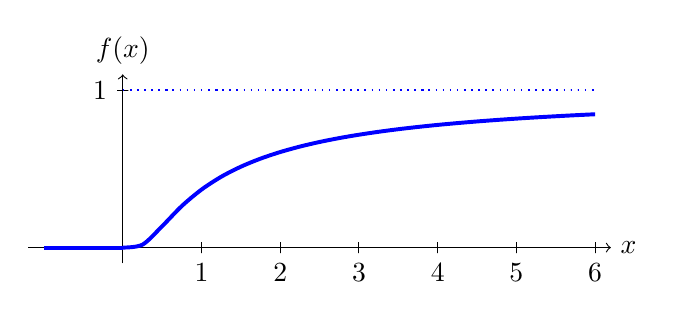
\begin{tikzpicture}{-1}{10}{0}{1.2}{1}

		\draw[->] (-1.2,0) -- (6.2,0) node[right] {$x$};
		\draw[->] (0,-0.2) -- (0,2.2) node[above] {$f(x)$};

		\draw (0,2) node (a) [fill = white,rectangle,inner sep = 0pt,minimum size = 0pt,minimum width=4pt,draw, label={left:$1$}] {};

		\draw[line width=0.5mm, scale=1, domain=-1:0, smooth, variable=\x, blue] plot ({\x},{0}) node[below right] {};
		\draw[line width=0.5mm, scale=1, domain=0.001:6, smooth, variable=\x, blue] plot ({\x},{2*exp(-1/\x)}) node[below right] {};
		\draw[line width=0.2mm, scale=1, domain=0:6, dotted, smooth, variable=\x, blue] plot ({\x},{2}) node[below right] {};

		\foreach \x in {1,2,3,4,5,6}
		\draw (\x,0) node[minimum width=0pt, minimum height=4pt, inner sep=0pt, draw, label={below:$\x$}] {};
	\end{tikzpicture}
\end{center}
Diese Funktion ist beliebig oft differenzierbar (auch in $x_0=0$) und es gilt:
\begin{equation*}
	f^{(n)}(0)=0 \quad\forall n\in\N
\end{equation*}
Für die Taylorreihe von $f$ bei $x_0=0$ gilt also $T_n(x)\equiv0$. Diese Funktion lässt sich also nicht einmal lokal durch ihr Taylorpolynom darstellen!
\begin{definition}{Analytische Funktionen}
	Eine beliebig oft differenzierbare Funktion, die sich lokal durch ihre Taylorreihe darstellen lässt, heißt \emph{analytisch}.
\end{definition}
\paragraph{Interessante Tatsache:}
Für Funktionen $f:U\rightarrow\C$ mit $U\subseteq \C$ eine offene Teilmenge, gilt:

Ist $f$ einmal komplex differenzierbar, ist sie bereits beliebig oft differenzierbar und analytisch!

Komplexe, analytische Funktionen nennt man auch homomorph.
